\documentclass[a4paper,12pt,twoside,openany]{report}

% Wzorzec pracy dyplomowej
% J. Starzynski (jstar@iem.pw.edu.pl) na podstawie pracy dyplomowej
% mgr. inż. Błażeja Wincenciaka
% Wersja 0.1 - 8 października 2016
%

\usepackage{polski}
\usepackage{helvet}
\usepackage[T1]{fontenc}
\usepackage{anyfontsize}
\usepackage[utf8]{inputenc}
\usepackage[pdftex]{graphicx}
\usepackage{tabularx}
\usepackage{array}
\usepackage[polish]{babel}
\usepackage{subfigure}
\usepackage{amsfonts}
\usepackage{verbatim}
\usepackage{indentfirst}
\usepackage{listings}
\usepackage[pdftex]{hyperref}


% rozmaite polecenia pomocnicze
% gdzie rysunki?
\newcommand{\ImgPath}{.}

% oznaczenie rzeczy do zrobienia/poprawienia
\newcommand{\TODO}{\textbf{TODO}}


% wyroznienie slow kluczowych
\newcommand{\tech}{\texttt}

% na oprawe (1.0cm - 0.7cm)*2 = 0.6cm
% na oprawe (1.1cm - 0.7cm)*2 = 0.8cm
%  oddsidemargin lewy margines na nieparzystych stronach
% evensidemargin lewy margines na parzystych stronach
\def\oprawa{1.05cm}
\addtolength{\oddsidemargin}{\oprawa}
\addtolength{\evensidemargin}{-\oprawa}

% table span multirows
\usepackage{multirow}
\usepackage{enumitem}	% enumitem.pdf
\setlist{listparindent=\parindent, parsep=\parskip} % potrzebuje enumitem

%%%%%%%%%%%%%%% Dodatkowe Pakiety %%%%%%%%%%%%%%%%%
\usepackage{prmag2017}   % definiuje komendy opieku,nrindeksu, rodzaj pracy, ...


%%%%%%%%%%%%%%% Strona Tytułowa %%%%%%%%%%%%%%%%%
% To trzeba wypelnic swoimi danymi
\title{Wycena działek budowlanych z wykorzystaniem uczenia maszynowego}

% autor
\author{Katarzyna Kolasa}
\nrindeksu{284919}

\opiekun{dr hab. inż.  Paweł Piotrowski}
\terminwykonania{1 lutego 2022} % data na oświadczeniu o samodzielności
\rok{2022}


% Podziekowanie - opcjonalne
%\podziekowania{\noindent
{\Large Podziękowania}
\bigskip

Dziękujemy bardzo serdecznie wszystkim, a w szczególności Rodzinom i~Unii Europejskiej...

\bigskip

{\raggedleft
Zdolny Student i Pracowity Kolega

}

}

\miasto{Warszawa}
\uczelnia{POLITECHNIKA WARSZAWSKA}
\wydzial{WYDZIAŁ ELEKTRYCZNY}
\instytut{INSTYTUT ELEKTROENERGETYKI}
%\instytut{INSTYTUT ELEKTROTECHNIKI TEORETYCZNEJ\linebreak[1] I~SYSTEMÓW INFORMACYJNO-POMIAROWYCH}
\zaklad{ZAKŁAD SIECI I SYSTEMÓW ELEKTROENERGETYCZNYCH}
% \zaklad{ZAKŁAD ELEKTROTECHNIKI TEORETYCZNEJ\linebreak[1] I~INFORMATYKI STOSOWANEJ}
%\kierunekstudiow{INFORMATYKA}

% domyslnie praca jest inzynierska, ale po odkomentowaniu ponizszej linii zrobi sie magisterska
%\pracamagisterska
%%% koniec od P.W

\opinie{%
  \newpage
\begin{center}
 {\large\bf  Opinia} \\
o pracy dyplomowej magisterskiej wykonanej przez dyplomanta\\
{\bf Zdolnego Studenta i Pracowitego Kolegę} \\
 Wydział Elektryczny, kierunek Informatyka,  Politechnika Warszawska\\
Temat pracy\\
\textit{\bf
TYTUŁ PRACY DYPLOMOWEJ
}\\
\end{center}
\medskip
\noindent
Promotor: {\bf dr inż. Miły Opiekun}\\
Ocena pracy dyplomowej: {\bf bardzo dobry}

\medskip

\centerline{\bf Treść opinii}
   Celem pracy dyplomowej panów dolnego Studenta i Pracowitego Kolegi  było
opracowanie systemu pozwalającego symulować  i opartego o oprogramowanie o
otwartych źródłach (ang. Open Source). Jak piszą Dyplomanci, starali się opracować
system, który łatwo będzie dostosować do zmieniających się dynamicznie wymagań,
będzie miał niewielkie wymagania sprzętowe i umożliwiał dalszą łatwą rozbudowę oraz
dostosowanie go do potrzeb.
Przedstawiona do recenzji praca składa się z krótkiego wstępu jasno i
wyczerpująco opisującego oraz uzasadniającego cel pracy, trzech rozdziałów (2-4)
zawierających opis istniejących podobnych
rozwiązań, komponentów rozpatrywanychjako kandydaci do
tworzonego systemu i wreszcie zagadnień wydajności wirtualnych
rozwiązań. Piąty rozdział to opis przygotowanego przez
Dyplomantów środowiska obejmujący opis konfiguracji
środowiska oraz przykładowe ćwiczenia laboratoryjne. Ostatni
rozdział pracy to opis możliwości dalszego
rozwoju projektu. W ramach przygotowania pracy Dyplomanci zebrali i przedstawili w
bardzo przejrzysty sposób duży zasób informacji, co świadczy o dobrej orientacji
w nowoczesnej i ciągle intensywnie rozwijanej tematyce stanowiącej
zakres pracy i o umiejętności przejrzystego przedstawienia tych
wyników. Praca zawiera dwa dodatki, z których pierwszy obejmuje wyniki
eksperymentów i badań nad wydajnością, a drugi to źródła
skryptów budujących środowisko.

 Dyplomanci dość
dobrze zrealizowali postawione przed nimi zadanie,
wykazali się więc umiejętnością zastosowania w praktyce wiedzy
przedstawionej w rozdziałach 2-4.  Uważam, że cele postawione w założeniach pracy zostały pomyślnie
zrealizowane. Proponuję ocenę bardzo dobrą (5).

\vskip 1cm
{
\raggedleft
(data, podpis)\kern1cm

}
  \newpage
  \newpage
\begin{center}
 {\large\bf  Recenzja } \\
pracy dyplomowej magisterskiej wykonanej przez dyplomanta\\
{\bf Zdolnego Studenta i Pracowitego Kolegę} \\
 Wydział Elektryczny, kierunek Informatyka,  Politechnika Warszawska\\
Temat pracy\\
\textit{\bf
TYTUŁ PRACY DYPLOMOWEJ
}\\
\end{center}
\medskip
\noindent
Recenzent: {\bf prof. nzw. dr hab. inż. Jan Surowy}\\
Ocena pracy dyplomowej: {\bf bardzo dobry}
\medskip


\centerline{\bf Treść recenzji}
   Celem pracy dyplomowej panów dolnego Studenta i Pracowitego Kolegi  było
opracowanie systemu pozwalającego symulować  i opartego o oprogramowanie o
otwartych źródłach (ang. Open Source). Jak piszą Dyplomanci, starali się opracować
system, który łatwo będzie dostosować do zmieniających się dynamicznie wymagań,
będzie miał niewielkie wymagania sprzętowe i umożliwiał dalszą łatwą rozbudowę oraz
dostosowanie go do potrzeb.
Przedstawiona do recenzji praca składa się z krótkiego wstępu jasno i
wyczerpująco opisującego oraz uzasadniającego cel pracy, trzech rozdziałów (2-4)
zawierających bardzo solidny i przejrzysty opis: istniejących podobnych
rozwiązań (rozdz. 2), komponentów rozpatrywanychjako kandydaci do
tworzonego systemu (rozdz. 3) i wreszcie zagadnień wydajności wirtualnych
rozwiązań, zwłaszcza w kontekście współpracy  kilku elementów
 sieci (rozdział 4). Piąty rozdział to opis przygotowanego przez
Dyplomantów środowiska obejmujący opis konfiguracji
środowiska oraz przykładowe ćwiczenia laboratoryjne (5 ćwiczeń). Ostatni, szósty
rozdział pracy to krótkie zakończenie, które wylicza także możliwości dalszego
rozwoju projektu. W ramach przygotowania pracy Dyplomanci zebrali i przedstawili w
bardzo przejrzysty sposób duży zasób informacji o narzędziach, Rozdziały 2, 3 i 4 świadczą o dobrej orientacji
w nowoczesnej i ciągle intensywnie rozwijanej tematyce stanowiącej
zakres pracy i o umiejętności syntetycznego, przejrzystego przedstawienia tych
wyników. Drobne  mankamenty tej części pracy to zbyt skrótowe omawianie
niektórych zagadnień technicznych, zakładające dużą początkową wiedzę czytelnika
i dość niestaranne podejście do powołań na źródła.
Utrudnia to w pewnym stopniu czytanie pracy i zmniejsza jej wartość dydaktyczną
(a ta zdaje się być jednym z celów Autorów), ale jest zrekompensowane zawartością
merytoryczną. Praca zawiera dwa dodatki, z których pierwszy obejmuje wyniki
eksperymentów i badań nad wydajnością, a drugi to źródła
skryptów budujących środowisko. Praca
zawiera niestety dość dużą liczbę drobnych błędów redakcyjnych, ale nie wpływają
one w sposób istotny na na jej czytelność i wartość. W całej pracy przewijają
się samodzielne, zdecydowane wnioski Autorów, które są wynikiem własnych i
oryginalnych badań.  Rozdział 5 i dodatki pracy przekonują mnie, że Dyplomanci dość
dobrze zrealizowali postawione przed nimi zadanie. Pozwala to stwierdzić, że
wykazali się więc także umiejętnością zastosowania w praktyce wiedzy
przedstawionej w rozdziałach 2-4. Kończący pracę rozdział szósty świadczy o
dużym (ale moim zdaniem uzasadnionym) poczuciu własnej wartości i jest
świadectwem własnego, oryginalnego spojrzenia na tematykę przedstawioną w pracy
dyplomowej. Uważam, że cele postawione w założeniach pracy zostały pomyślnie
zrealizowane. Proponuję ocenę bardzo dobrą (5).

\vskip 1cm
{
\raggedleft
(data, podpis)\kern1cm

}
}

\streszczenia{
  \newpage
\begin{center}
\large \bf
TYTUŁ PRACY DYPLOMOWEJ
\end{center}

\section*{Streszczenie}
Praca składa się z krótkiego wstępu jasno i
wyczerpująco opisującego oraz uzasadniającego cel pracy, trzech rozdziałów (2-4)
zawierających opis istniejących podobnych
rozwiązań, komponentów rozpatrywanychjako kandydaci do
tworzonego systemu i wreszcie zagadnień wydajności wirtualnych
rozwiązań. Piąty rozdział to opis  środowiska obejmujący opis konfiguracji
środowiska oraz przykładowe ćwiczenia laboratoryjne. Ostatni
rozdział pracy to opis możliwości dalszego
rozwoju projektu. 

\bigskip
{\noindent\bf Słowa kluczowe:} praca dyplomowa, LaTeX, jakość

\vskip 2cm


\begin{center}
\large \bf
THESIS TITLE
\end{center}

\section*{Abstract}
This thesis presents a novel way of using a novel algorithm to solve complex
problems of filter design. In the first chapter the fundamentals of filter design
are presented. The second chapter describes an original algorithm invented by the
authors. Is is based on evolution strategy, but uses an original method of filter
description similar to artificial neural network. In the third chapter the implementation
of the algorithm in C programming language is presented. The fifth chapter contains results
of tests which prove high efficiency and enormous accuracy of the program. Finally some
posibilities of further development of the invented algoriths are proposed.

\bigskip
{\noindent\bf Keywords:} thesis, LaTeX, quality

\vfill
}

\begin{document}
\maketitle

\chapter{Wstęp do problemu wyceny działek budowlanych}

\section{Wprowadzenie}
Na początku przedstawione zostaną pojęcia działki budowlanej i wyceny, by doprecyzować temat niniejszej pracy oraz sprawdzić, czy z formalnych definicji można zaczerpnąć na potrzeby dalszych rozważań.//
W drugiej części tego rozdziału przeanalizowane zostanie, w jaki sposób i przez kogo zagadnienie wyceny działek budowlanych jest już obecnie realizowane, a w szczególności, jakie narzędzia są do tego wykorzystywane


\section{Definicja działki budowlanej}
Jako materiały źródłowe przywołane będą poniżej polskie akty prawne, które definiują pojęcia działki, działki budowlanej, a także nieruchomości. Pojęcie nieruchomości jest najbardziej ogóle, jednak istotne dla dalszych definicji, dlatego zostanie poruszone na początku.//

 Polski Kodeks Cywilny definiuje nieruchomości jako
\textit { części powierzchni ziemskiej stanowiące odrębny przedmiot własności (grunty), jak również budynki trwale z gruntem związane lub części takich budynków(...)} \cite{KC}
Definicja jest ogólna, ale wskazuje już na zagadnienie własności, które może się okaząć później istotne jako potencjalny parametr dla modelu. Ponadto różnicuje grunty oraz budynki. Budynki same w sobie nie są przedmiotem tej pracy, jeśli zaś chodzi o rodzaje działek gruntowych, dzieli się jem.in  na działki rolne i siedliskowe (tutaj zabudowania to różnego rodzaju budynki związane z produkcją rolną, rownież zabudowania mieszkalne, jeśli nie są rodzielne od budynków gospodarczych), budowlane przeznaczone na zabudowę mieszkaniową,  inwestycyjne (przemysłowe), rekreacyjne (tutaj jako grunty zabudowane wystapić moga np domki na terenie ogrodów działkowych, które nie muszą być uzbrojone), leśne. \cite{RMRPiTegb}\\


Pojęcie działki budowlanej doprecyzowane jest w kilku aktach prawnych, np w Ustawie o planowaniu i zagospodarowaniu przestrzennym, która definiuje ją jako \textit {nieruchomość gruntową lub działkę gruntu, której wielkość, cechy geometryczne, dostęp do drogi publicznej oraz wyposażenie w urządzenia infrastruktury technicznej spełniają wymogi realizacji obiektów budowlanych(...)}
\cite{Uopizp}
Z tej definicji wynika, że na działce budowlanej można zgodnie z prawem wznieść nieruchomość. Wskazuje równiez na powierzchnię, kształ, dojazd, infrastrukturę jako istotne cechy działki, któ©e będą potencjalnymi parametrami modelu w dalszej części pracy.\\

Tymaczesm Ustawa o gospodarce nieruchomościami  definiuje działkę budowlaną podobnie, ale jako \textit {zabudowaną działkę grutu}\cite{Uogn}. Definicja nie jest więc spójna. 
Na potrzeby tej pracy działkę budowlaną będziemy postrzegać w pierwszym ujęciu -jako teren, na którym prawo dopuszcza postawienie nieruchomości. Zdecydowanie zabudowanie działki nie będzie jednak warunkiem koniecznym.
Potencjalny problem, jaki powstaje w tym miejscu, to czy zabudowane działki
będą klasykikowane jako domy, magazyny itd, czy jako działki budowlane.\\


Założeniem tej pracy jest skupienie się na działkach, czyli określenie wartości samego gruntu. W dalszej części pracy wskazane będzie, w jakim stopniu możliwe jest rozdzielenie ofert sprzedaży działek zabudowanych i niezabudowanych.\\


Co się tyczy dalszych warunków, jakie spełniać powinna działka budowlana, przeczytamy również: \\


 \textit {Działka budowlana przewidziana pod zabudowę budynkami przeznaczonymi na pobyt ludzi powinna mieć zapewnioną możliwość przyłączenia uzbrojenia działki lub bezpośrednio budynku do sieci wodociągowej, kanalizacyjnej, elektroenergetycznej i ciepłowniczej, (...) telekomunikacyjnej. 2. Za równorzędne z przyłączeniem do sieci elektroenergetycznej i ciepłowniczej uznaje się zapewnienie możliwości korzystania  z indywidualnych  źródeł  energii  elektrycznej  i ciepła(...)}\cite{RMI}

Ten fragment wskazuje na potencjalne parametry danych wejściowych w dalszej części pracy: dostępność mediów i możliwość przyłączenia do sieci.


Warto również zaznaczyć, że nawet jeśli w ogłoszeniu o sprzedaży dana działka będziw oznaczona jako budowlana, należy zweryfikować w  Miejscowym Planie Zagospodoarowania Przestrzennego, czy w istocie nadaje się pod zabudowę. Te plany dostepne są w internecie, w formacie interaktywnej mapy, mapy pdf, oraz - przede wszystkim - jako tekst uchwały samorządu. 
Ponieważ na portalach ogłoszeniowych można podać przybliżoną lokalizację działki, ani administrator portalu, ani użytkownik nie jest w stanie zweryfikować, czy podane przez ogłoszeniodawcę przeznaczenie działki jest zgodne z prawdą, z tego względu już na wstępnie trzeba liczyć się z potencjalnie źle oznaczonymi danymi.



\section{Definicja wyceny nieruchomości}
W tej sekcji sprawdzone zostanie, jak można rozumieć pojęcie wyceny, i co można zaczerpnąć z formalnego opisu tego pojęcia. Na wstępie zaznaczyć należy, że teksty źródłowe (akty prawne) traktują  o wycenianiu nieruchomości w ogóle, nie odnoszą się do przypadku działki bądź działki budowlanej w szczególności.


W Dzienniku Ustaw czytamy, że \textit{określanie wartości nieruchomości następuje przy zastosowaniu poszczególnych podejść, metod, technik wyceny} \cite{OPRM}. W takim ujęciu wycena służy określaniu wartości nieruchomości, a \textit{wycena} i \textit{określenie wartości} nie są wyrażaniami synonimicznymi, ale na tyle bliskoznaczymi, że na potrzeby tej pracy w dalszej części będą traktowane równoważnie.\\
Cytowane rozporządzenie precyzuje dalej szereg środków, które umożliwiają realizację zadania, jakim jest wycena czyli \textit {określenie wartości prawa własności lub innych praw do nieruchomości}.

Wyceny nieruchomości dokonuje (szczególnie jako biegły) rzeczoznawca majątkowy - opnia wydana na piśmie to operat szacunkowy\cite{Operat}; oprócz tego trudnić się może zajmować się m.in. doradztwem w zakresie rynku nieruchomości\cite{Operat2}. By osiągnąć ten cel, może zastosować podejście porównawcze, dochodowe, mieszane oraz kosztowe. Każde podejście jest realizowane za pomocą odrębnych metod, z którymi z kolei wiążą się różne techniki.
Wyróżnione zostają następujące podejścia:
\begin{itemize}

\item dochodowe - w tym podejściu zasadniczą rolę odgrywa znajomość dochodów uzyskiwanych lub możliwych do uzyskania z nieruchomości, do wyceny można zaś zastosować analizę stawek rynkowych czynszów i dzierżawy, albo analizę dochodów uzyskiwanych z działalności w podobnych nieruchomościach.

To podejście nie będzie miało zastosowania w dalszej częsci pracy ponieważ informacje dotyczące dochodów z nieruchomości nie są ogólnodostępne.


\item mieszane - stosuje się analizę kosztów robót budowlanych - remontu, rozbudowy, itp, analizę kosztów likwidacji  -które znowu nie są ogólnodostepne albo metodę wskaźników szacunkowych gruntów, która z kolei dotyczy gruntów leśnych i rolnych, więc nie będących przedmiotem tej pracy


\item kosztowe - trzecie podejście do wyceny nieruchomości jest realizowane poprzez określanie\ textit{ kosztów odtworzenia} lub \textit {zastąpienia}  części skłądowych gruntu częściami o takiej samej funkcji; przy tym podejściu może wystaąpić sytuacja, gdy wartość nieruchomości - ze względu na wysoki koszt przywrócenia jej do stanu umożliwiającego użytkowanie zgodnie z przeznaczniem- będzie liczbą ujemną.

\item porównawcze - jest czwartym i ostatnim podejściem, z którym wiążą się metody \textit{porównywania parami} - wycenianą nieruchomośc porównuje się kolejno z podobnymi nieruchomościami, które były przedmiotem obrotu rynkowego, \textit{korygowania ceny średniej} - gdzie wylicza się średnią cenę transakcyjną z przynajmniej kilkunastu podobnych nieruchomości, a następnie koryguje o poszczególne cechy nieruchomości, \textit {analizy statystycznej} - ustawa nie przybliża jednak konkretnych metod.

\end{itemize}


Podejście porównawcze opisane powyżej jest najbliższe zastosowanemu do przeprowadzenia wyceny w dalszej części pracy, gdzie danymi wejściowymi dla sieci neuronowej są dane o  cenach i cechach nieruchomości zebrane z dostępnych w internecie ofert. \\
W metodzie porównawczej uwzględniane są jednak ceny transakcyjne, do których dostęp mają osoby lub instytucje biorące bezpośredni udział w transakcjach kupna-sprzedaży oraz biura nieruchomości. Korzystający z tej metody powinnini znać również warunki zawarcia tych transakcji  oraz to, jak cechy danej nieruchomości wpłynęły na cenę transakcyjną, np szczególną ostrożność trzeba zaś przyłożyć do cen związanych z przetargami.\\
Ceny powszechnie dostępne to cenyofertowe  podawane w ogłoszeniach o sprzedaży nieruchomości, które są cenami rynkowymi, nie koniecznie są jednak cenami transakcyjnymi.
Powyżej nakreślone zostało pojęcie wyceny w formalnym, prawnym ujęciu, oraz w jaki sposób może być ona realizowana przez rzeczoznawcę.


\section {Istniejące rozwiązania}
Istnieje na rynku przynajniej kilka rozwiązań, wspierających proces wyceny nieruchomości.
Portale internetowe (na przykład skup.io, ceny.szybko.pl) oferują usługę kalkulatora wartości nieruchomości. Aby dokonać wyceny, należy wprowadzić m.in informacje o adresie, roku budowy, metrażu, liczbie pokoi, numerze piętra, subiektywnie ustalonym standardzie, udogodnieniach. Obie wspomniane strony w domyślnym formularzu przeznaczonym do wyceny domu/mieszkania oferują zaznaczenie opcji, że na sprzedaż jest działka, jednak nie powoduje to zmiany wygladu formularza. \cite{skup} \cite{cenyszybko}

Drugi ze wspomnianych portali w opisie swojej oferty wspomina o wykorzystaniu AVM (Automated valuation Model), Automatycznego Modelu Wyceny, który analizuje ceny transakcyjne i ofertowe oraz cechy konkretnej nieruchomości i oblicza rynkową wartość nieruchomości za pomocą modelu statystycznego. \\
Według Polskiej Federacji Stowarzyszeń Rzeczoznawców Majątkowych AMW to oparty na statystyce program komputerowy wykorzystujacy informacje z bazy cen transakcyjnych i cech nieruchomości do generowania wartości nieruchomości. Wspomaga pracę rzeczoznawcy i może posłużyć jako jedna z danych wejściowych, lecz nie może jednak zupełnie zastąpić oceny biegłego, m.in dlatego, że pomija tradycyjną wycenę opartą np na podejsciu dochodowym lub porównawczym i fizyczną, jakościową ocenę wykonywaną przez rzeczoznawcę. \cite{plfed}

Wykorzystanie sieci neuronowej jest jedną z dostępnych metod obliczeniowych podczas implementacji AMW \cite{AVMFigurska}, obok analizy regresji, analizy szeregów czasowych, modeli ważonych geograficznie, modeli symulacyjnych, algorytmów genetycznych itp. \cite{AMVbilozor}


\cite{szybko}AVM wspomniane jest np w dokumentacji sporządzonej przez Europejską Grupe Stowarzyszeń Rzeczoznawców Majątkowych (TEGOVA), która stwierdza, że zaawansowane modele statystyczne są najnowocześniejszą i najbardziej wyfarinowanymi AVM. \cite{AVM} 


Portal ceny.szybko.pl oferuje Heatmapę, która ma odzwierciedlać średni poziom cen w okolicy oraz dostęp do historii zmian cen w wybranej lokalizacji do 3 lat wstecz. \cite{szybko}, a strona otodom.pl Mapę Cen, która, za stroną \textit{jest budowana i aktualizowana na bieżąco od wielu lat, na podstawie danych płynących bezpośrednio z urzędów gmin i miast}\cite{otodom} i przedstawia mapę cen transakcyjnych stworzoną z parterem technologicznym PriceR, który na swojej stronie  oferuje jedynie wyceny mieszkań. \cite{pricer}

\section{Podsumowanie}

Z powyższch rozważań wynika, że problem wyceny dziełek budowlanych związany jest z zagadnieniem wyceny nieruchomości w ogóle. 
Na poziomie portalu z ogłoszeniami o sprzedaży działek nie można zweryfikować, jakie są faktyczne warunki zabudowy gruntu.
Ponadtwo, działka pasująca do definicji działki budowlanej może być zabudowana lub nie.
Formalnie -do celów urzędowych - wyceną działki budowlanej zajmuje się rzeczoznawca majątkowy. Dokonuje wyceny na podstawie znajomości rynku, a szczególnie cen transakcyjnych, które nie są informacjami ogólnodostepnymi. Rzeczoznawca ma do dyspozycji szereg metod i technik, jednak nie są one opisane na tyle szczegółowo, by można było z nich czerpać na potrzeby tej pracy, korzystać może również z narzędzi w rodzaju AMV, oferowanych przez szereg podmiotów, 





\chapter{Źródła danych wejściowych do modeli oraz ich charakterystyka}
 ----laska z Warmii 
 .2. Budowa automatycznego modelu wyceny
Wedãug SCHULZA i in. (2014, s. 134-135), budowa AVM powinna zaczĈþ sič od zapewnienia ciĈgãego,
nieprzerwanego dostčpu do rzetelnych i aktualnych danych. WiarygodnoĤþ AVM, obliczajĈcego
wartoĤþ rynkowĈ na podstawie modelowania matematycznego, podobnie jak w przypadku wyników
tradycyjnych wycen, zaleİna jest nie tylko od umiejčtnoĤci jego twórcy (MOORE 2006, s. 46), a
 ----

Dane o cenach transakcyjnych nierychomości są dostepne za opłątą. Publiczną bazą danych jest publicznych baz danych jest Rejestr Cen i Wartości Nieruchomości (RCiWN) 
https://stat.gov.pl/metainformacje/slownik-pojec/pojecia-stosowane-w-statystyce-publicznej/4491,pojecie.html

Dane wejściowe zebrane zostały z internetowych portali z ogłoszeniami o nieruchomościach. Wykorzystane zostały trzy serwisy o bezpłatnym, publicznym dostępie: domiporta, morizon, otodom.

\section{Charakterystyka portalu otodom.pl}
OTODOM - dodanie ogłoszenia płątne, może to zrobić osoba prywatna; min kwota to 30 dni za 70 zł; biuro nieruchomości - na portalu czytamy, że korzysta z nigo ponad 5 tys. pośredników \cite{otodom_o_nas}\\

W pierwszym kroku trzba wybrać przedmiot ogłozenia (mieszkania, domy, pokoje, działkil loklae użytkowe, hale i magazyny, garaże) oraz rodzaj oferty( sprzedaż/wynajem), nastepnie strona się przeładowuje i w formularzu uzupełnić leży:\\
-cenę (zł, euro, usd, gbp)\\
-powierzchnię w m2\\
-typ ogłoszeniodawcy (właściciel/pośrenidk)\\
-lokalizację- wpisując nazwę miejscowości - po wpisaniu lokalizacja jest podana na mapie interaktywnej\\
-opis\\
\\
Dodatkowe informacje, jakie można dodać, to:\\
-dzielnica oraz ulica/osiedle\\
-typ działki (budowlana, rolna, rekreacyjna, pod inwerstycję, leśna, rolno-budowlana, siedliskoa, inna)\\
-wymiary (w dowolnym formacie - pole tekstowe)\\
ogrodzenie (tak/nie)
-położenie (miasto, pod miastem, wieś)\\
-media (prąd, telefon, oczyszczalnia, woda, kanalizacja, gaz, szambo) - wielokrotnego wyboru)\\
-dojazd (nieutwardzony, utwardzonyu, asfaltowy)\\
-okolica (las, góry, jezioro, morze, otwarty teren)\\

\section{Charakterystyka portalu domiporta.pl}
obowiązkowe:\\
-można zaimportować ogłoszenie z innego portalu\\
-rynek(wtórny/pierwotny)\\
-rodzaj transakcji (sprzedaż/wynejem)\\
-rodzaj nieruchomości (mieszkanie, dom, działka, lokal użytkowy, garaż, magazyn)\\
-powierzchnia (w m2)\\
-cena\\
\\
Po wybraniu opcji 'działka' i 'sprzedaż' pojawia się obowiazakowe pole \\
-typ działki (budowlana, komercyjna, leśna, leśna z prawem budowy, przemysłowo-handlowa, rekreacyjna, rolna, siedliskowa, inwestycyjna, gospodarstwo rolne, inna)\\
-cena (można wybrać walutę (pln, euro, usd)\\
-można odznaczyć pole 'cana do negocjacji'\\
\\\\
W seekcj lokazlizacja obowiązkowe jest przynajmniej podanie nazwy miejscowości.\\
Mzna cislić kod pocztowy, dizlenicę, osiedle, ulcę, nr domu
wybrane wartości odzwierciedlane są na internktywnej mapie w formulazu

Reszta informacji jest nieobowiażkowa; to .in. pola:
opis, dostepna od, kształt działki,
-kanalizacja (brak, szambo, miejska, oczyszczlania) -jednokrotnego wyboruu
-ogrodzenie działki (brak, siatka, drewniane, murowane, żywopłot, metalowe, inne) - jednokrotnego wyboru\\
-droga dojazdowa(asfaltowa, utwardzona, polna, brak)- jednokrotnego wyboru\\
-media(brak, gaz, proąd, siłą, woda) - wielokrotnego wyboru\\
-okolica (apteka, autobus, bazarek osiedlowy, centrum handlowe, kolej podmiejska, las, metro, niska zabudowa, park, PKP< plac zabaw, poczta, policja, przedszkole, przychodnia, szkołą, tramwaj, żłobek)\\

Najtańsza oferta za ogłoszenie to 49zł za 30 dni dla osoby prywantnej; aganecja nieruchomości mogą wystawić ogłoszenie za od 10,9 zł do 0,3 zł, nie jest podane, jak długo w tej ofercie byłoby wyświetlane ogłoszenie.


\section{Charakterystyka portalu morizon.pl}
Po wybraniu rodzaju i przedmiotu oferty (sprzedaży działki) obowiązkowe jest wskazanie:\\
-typu działki (rolna, budowlana, budowlaba-jednorodzinna, budowlana-wielorodzinna leśna, rekreacyjna, siedlisko, przemysłowa, handlowo-usługowa)\\

-powierzchni (w m2)\\
-ceny (w zł, euro, uds) z możliwości zaznaczenia opcji 'do negocjacji'\\
-tytułu i opisu ogłoszenia
-lokalizacji -obowiazkowo nalezy wybrać z rozwijanych list: województwo, powiat/miasto, gminę/dizlenicę
Dodatkowo można dodać miejscowość, ulicę, nr działki.\\
Wybrane wartości pokazane są na interaktywnej mapie w formularzu.\\
\\

Dodatkowo można dodać jako informacje szczegółowe:\\
-kanalizacja (miejska, szambo, brak, oczyszczlania)- jednokrotego wybotu\\
-szerokość i długość działki w metrach\\
-ogrodzenie (murowane, drewniane, siatka, brak, żywopło, metalowe/kute, inne, betonowe)\\
-droga dojazdowa (asfaltowa/betonowa, brk, utwardzona, nieutwardzona)\\
-media (prąd, woda, telefon, siła, gaz) - wielokrotnego wyboru\\
-dostępne od (miesiąc, rok)\\

Za ołatą można to samo ogłoszenie opbublikowac na kilku innych portalanach ( Gratka.pl, Domy.pl, Oferty.net, Bezposrednie.com, Nportal.pl, Onet, Mitula i Trovit. )\\

------------------------------------
\section{Podsumowanie}

Dane wejściowe zawieraja zawsze cenę, przy czym nie jest to cena transakcyjna - co warunkuje to, że wszelkie próby wyceny poprzez sieci neuronowe nie będa w stanie okteslić faktycznej wartości nieruchomości.
Wspólne są cena, powierzchnia, lokalizacja (może być przybliżona.\\

Dane wejściowe to: liczby oraz tekst.\\


Na portalach, z których pochodzą dane, nie ma dostępnych narzędzi, by odfiltrować oferty w których jako działki budowlane zabudowane oraz niezabudowane nie są rozdzielone- co wiązać się może z zawyżoną ceną w stosunku do grutnów niezabudowanych o podobnych paramtrach.
Oferty sprzedaży domów, magazynów itp są osobną kategorią.


\huge{Zastosowane metody pozyskiwania danych oraz przygotowania danych wejściowych}

 
\normalsize 
Pierwszym krokiem było zebranie danych o miastach w Polsce.
Zródłem byłą strona https://www.polskawliczbach.pl/Miasta'. Z której zebrane zostały informacje w formacie ['Warszawa', 'powiat Warszawa', 'mazowieckie', '1 790 658', '517,2 km²']
i zapisane do jednego pliku, w porzadku od miasta z największą liczbą ludności do miasta z najmniejszą liczbą ludnosci (['Koźminek', 'powiat kaliski', 'wielkopolskie', '1 978', '-']).
Wszystkich zapisanych miast jest 951.\\

W następnym kroku przygotowany został skrypt do przeglądania i zapisywania danych ze stron internetowych - webscrapingu.
Wykorzystane do tego została bibliteka języka Python - beautifulSoup.

Co robił ten skrypt

-iteration\_preprocessing uruchamiany był z argumentem - nazwą portalu\\
-wstawiał po kolei miasta do linku właściwego dla portalu -w pliku konfiguracyjnym miał zapisane linki do stron z działkami w danym miejście jako templatki\\
-dla danego miasta zapisywał wszystkie linki do poszczeglnych ofert - przy czym sprawdzał, czy nie ma koljenych stron (z kontuacją listy ofert dla wybranego miejsca); funkcja wyszukująca oferty jest inna dla każdego portalu\\
-następnie przeglądał kazdą z ofert dla miasta, wywołując funkcję collect\_info\_about\_plot z argumentami m.in nazwą portalu oraz linkiem do strony i zbierał klubowe informacje\\
-dla każdego portalu te informacje ukryte były w nieco inny sposób - konieczne było najpierw sprawdzenie (inspekcja) w przeglądarce, by odkryć, jak otagowane?? w cssss??? są konrentne informacje; zależnie od nazwy portalu wywoływany był inny Prser\\
-na początku tego parsera nie było, - było szybciej - ale dodałam, żeby coś zrobić obiektowo \\
-problem: są ukryte, dodatkowo zmieniają się z czasem; ponazywane sa nieintuicyjnie i konkretne elelmtnyu czasem można odróżnić np po nazwie stylu...\\
-czyszczenie z html\\
-
--obsługa błędów - brak, ofeta pomijana\\
-dane o ofertach z wybrnego miasta zapisywane były do jednego pliku, max 100 ofert w jedym (tylko dla Warszawy tworzone było kilka plików)

\begin{verbatim}
collect_data_about_plot zwracało:
    result_json = {
        "city": city,
        "price": price,
        "area": area,
        "features": features,
        "description": description,
        "coordinates": coordinates,
        "offer_link": plot_sales_offer,
    }
do 
\end{verbatim}



\chapter{Analiza statystyczna potencjalnych danych wejściowych do modeli wraz z ich wyborem}
Analiza bla bla bla.
Wybrane te i te.
\chapter{Projekt i implementacja narzędzia do wyceny działek budowlanych}
Zaimpelmentowałam to tak i siak.
\chapter{Wykonanie wycen działek budowlanych oraz analiza otrzymanych wyników}
Działki a i b i c wycenione zostały tak i siak
\chapter{Podsumowanie i wnioski}

-------------------------------------
\chapter{Pozostałość ze starej pracy}

\section{Historia}

Rozdziały \ref{sectionSteganografiaWObiektachMultimedialnych} oraz 
\ref{chapterSteganografiaWRuchuTCPIP} opisują nowoczesne podejście do 
steganografii wykorzystujące współczesne kanały informacyjne. 
\section{Schemat komunikacji steganograficznej}
\label{sectionSchematKomunikacjiSteganograficznej}
 Ma on pełen wgląd do przekazywanych 
informacji, więc może przechwycić wszelkie przekazywane tajemnice, a dodatkowo w 
razie podejrzeń może nie dopuścić do komunikacji\footnote{podejrzana informacja 
jest tu analogią do stosowania kryptografii przez więźniów}. W takim przypadku w 
celu przekazania ważnych informacji \tech{A} i \tech{B} muszą posłużyć się 
pewnego rodzaju podstępem. 
\begin{figure}[!htbp]
	\begin{center}
\centering
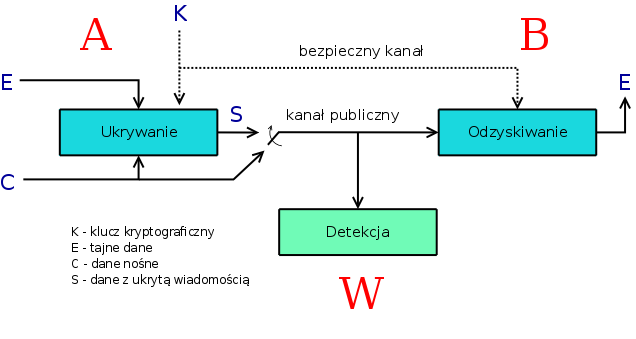
\includegraphics[scale=0.4]{\ImgPath/rys/schemat_komunikacji.png}
\end{center}
	\caption{Schemat komunikacji steganograficznej}
	\label{schematKomunikacji}
\end{figure}

Przedstawioną tak sytuację pokazuje rysunek 
\ref{schematKomunikacji}\footnote{sporządzony na podstawie 
\cite{schematKomunikacjiPrzypis}, rysunek 1, strona 3}. \tech{A} próbuje 
przesłać tajną informację \tech{E} do \tech{B}. Można tu wykorzystać metody kryptografii symetrycznej (ustalony 
klucz kryptograficzny \tech{K}) lub niesymetrycznej (klucz publiczny 
\tech{K}$_{pub}$ i klucz prywatny \tech{K}$_{pryw}$).

\section{Metody tworzenia steganografii oraz rodzaje ukrytych kanałów}
 W większości przypadków występujących w rzeczywistych sieciach i 
systemach, numery wygenerowane przy pomocy \tech{Shushi} nie byłyby rozróżnialne 
od numerów wygenerowanych przez stos sieciowy systemu.

\begin{tabular}{c|cc}
pierwsza kolumna & druga & trzecia \\ \hline
1 & 2 & 3 \\
a & b & c \\
\end{tabular} 

\begin{equation}
 E = m c^2 \label{einstein}
\end{equation}



\appendix
\chapter{Porównanie numerów ISN jądra Linux i modułu Shushi}
\begin{figure}[!htbp]
	\begin{center}
\centering
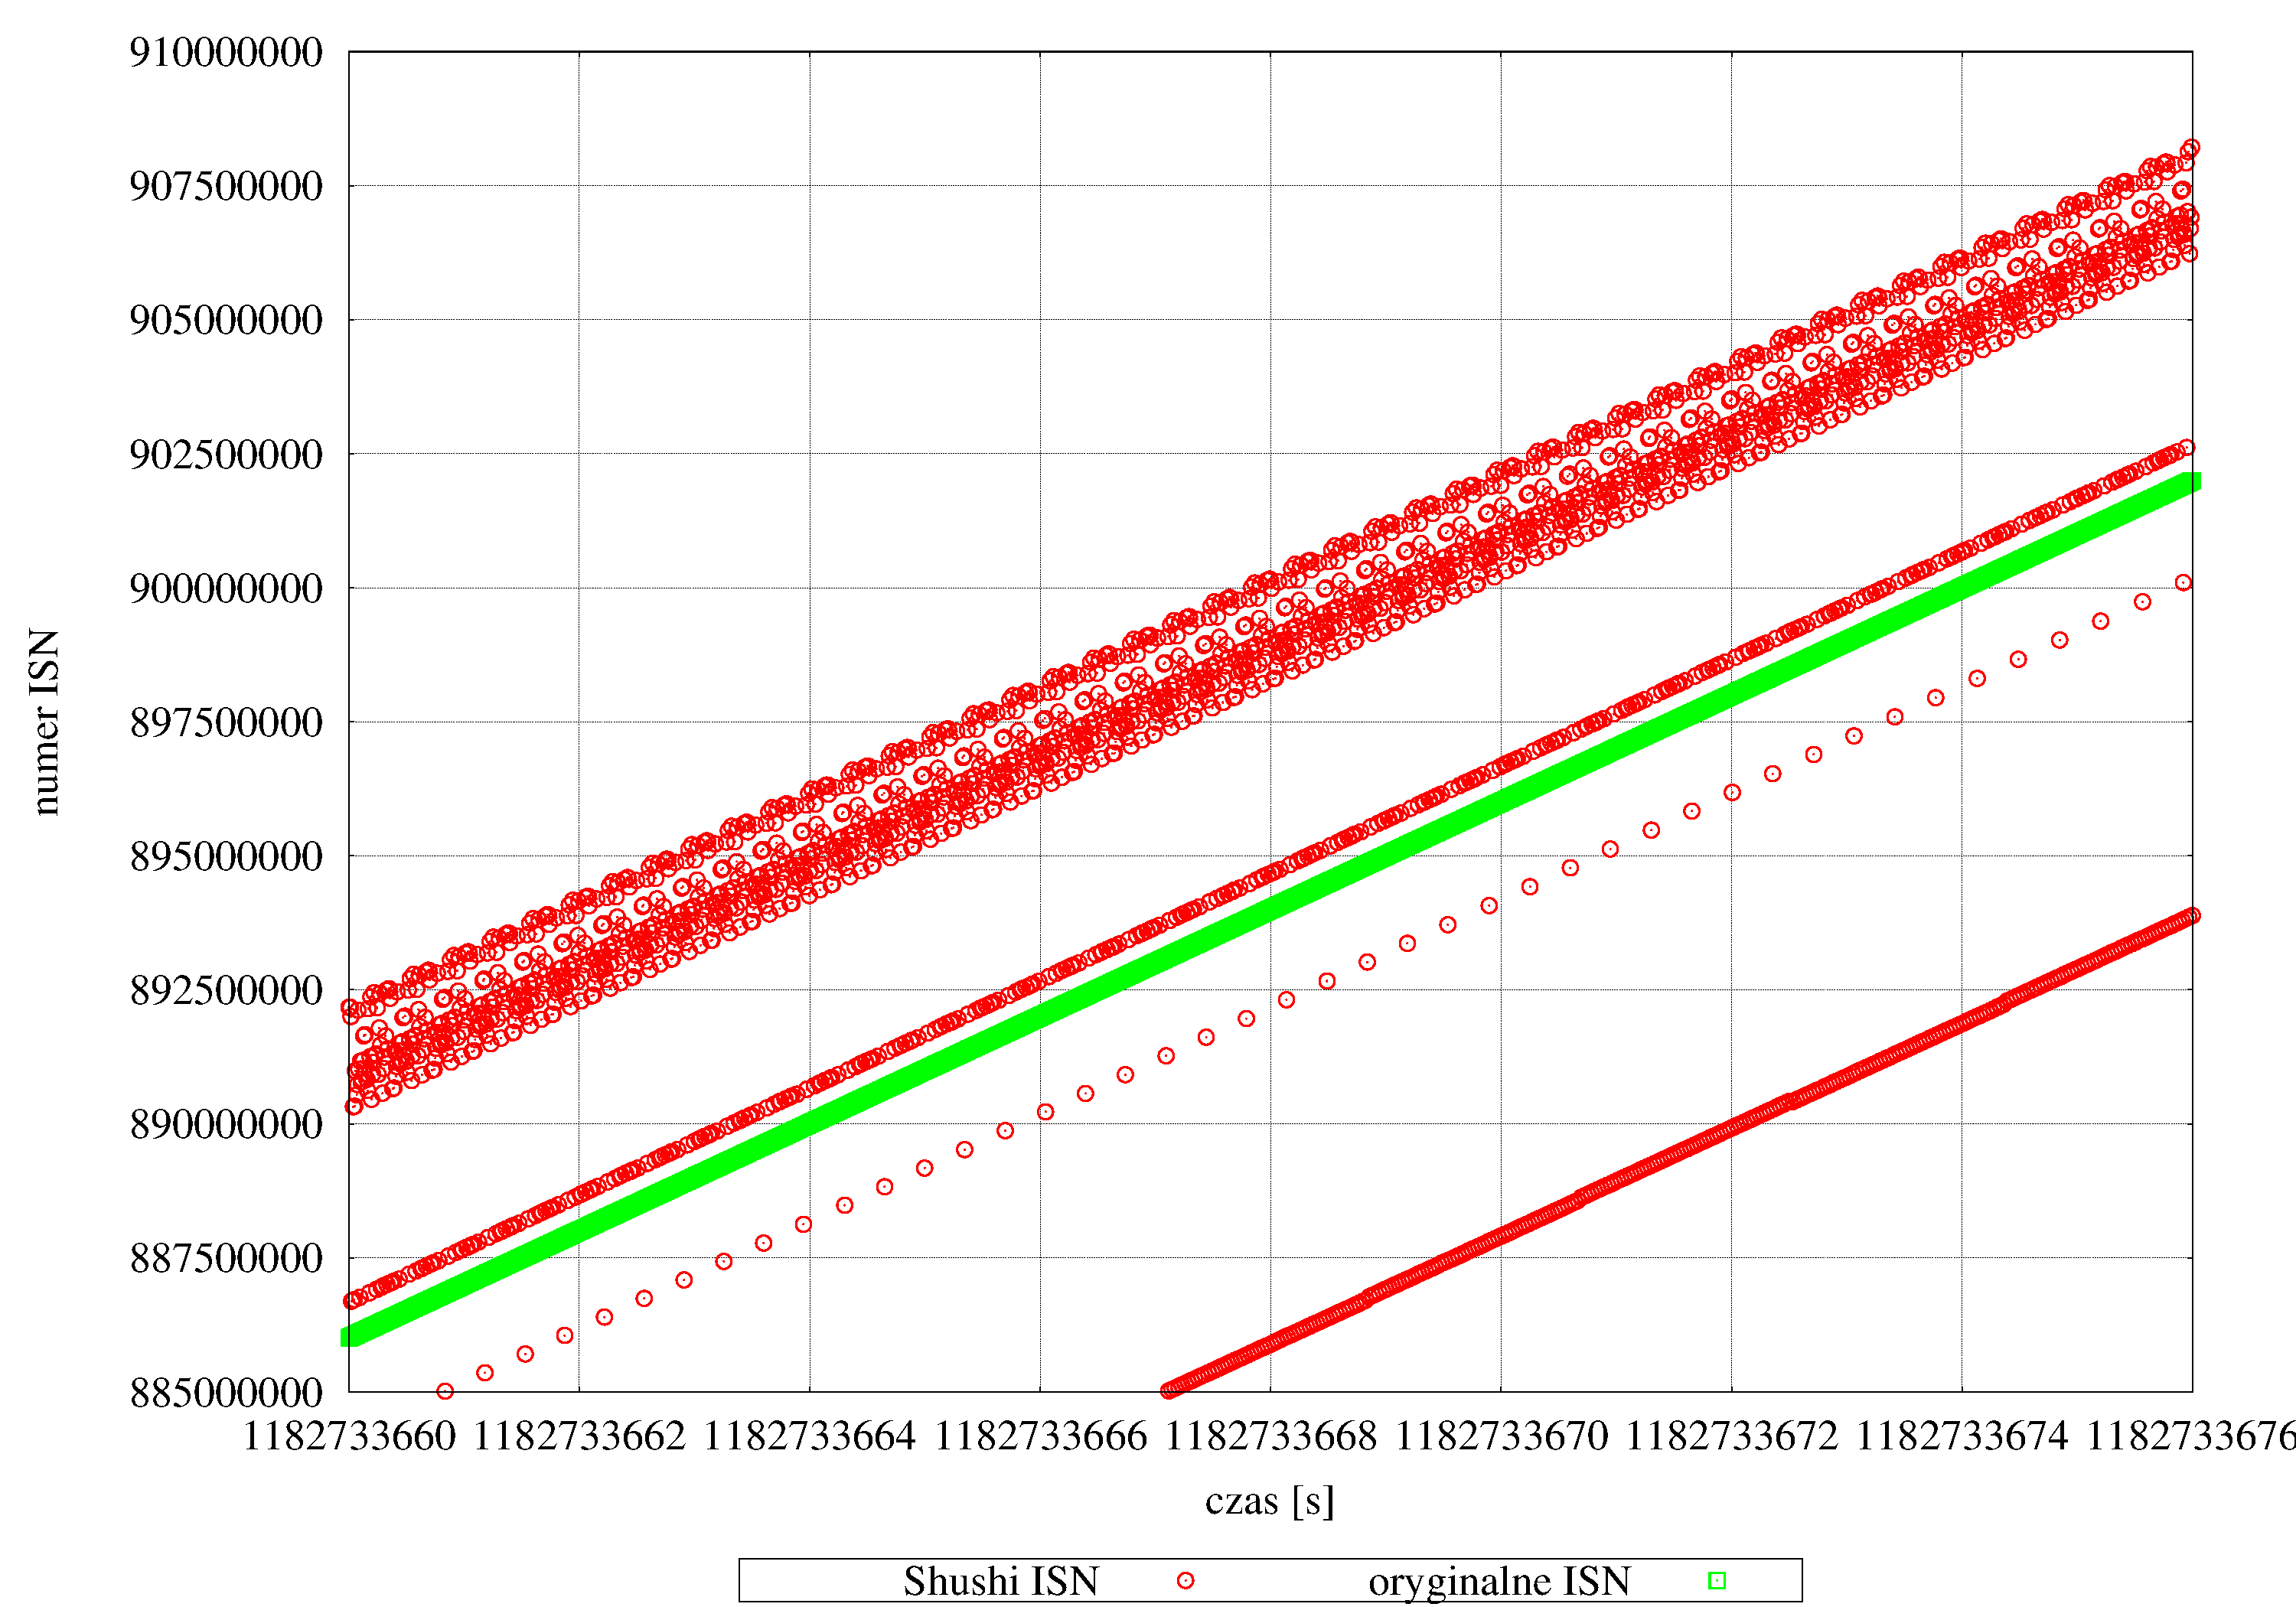
\includegraphics[scale=0.21]{\ImgPath/rys/IPPortConstData.pdf}
\end{center}
	\caption{Numery ISN wygenerowane przez jądro oraz \tech{Shushi}, stałe 
numery IP oraz porty TCP, stałe dane dla \tech{Shushi}, serie po około 2800 
próbek.}
	\label{IPPortConstData}
\end{figure}

\begin{figure}[!htbp]
	\begin{center}
\centering
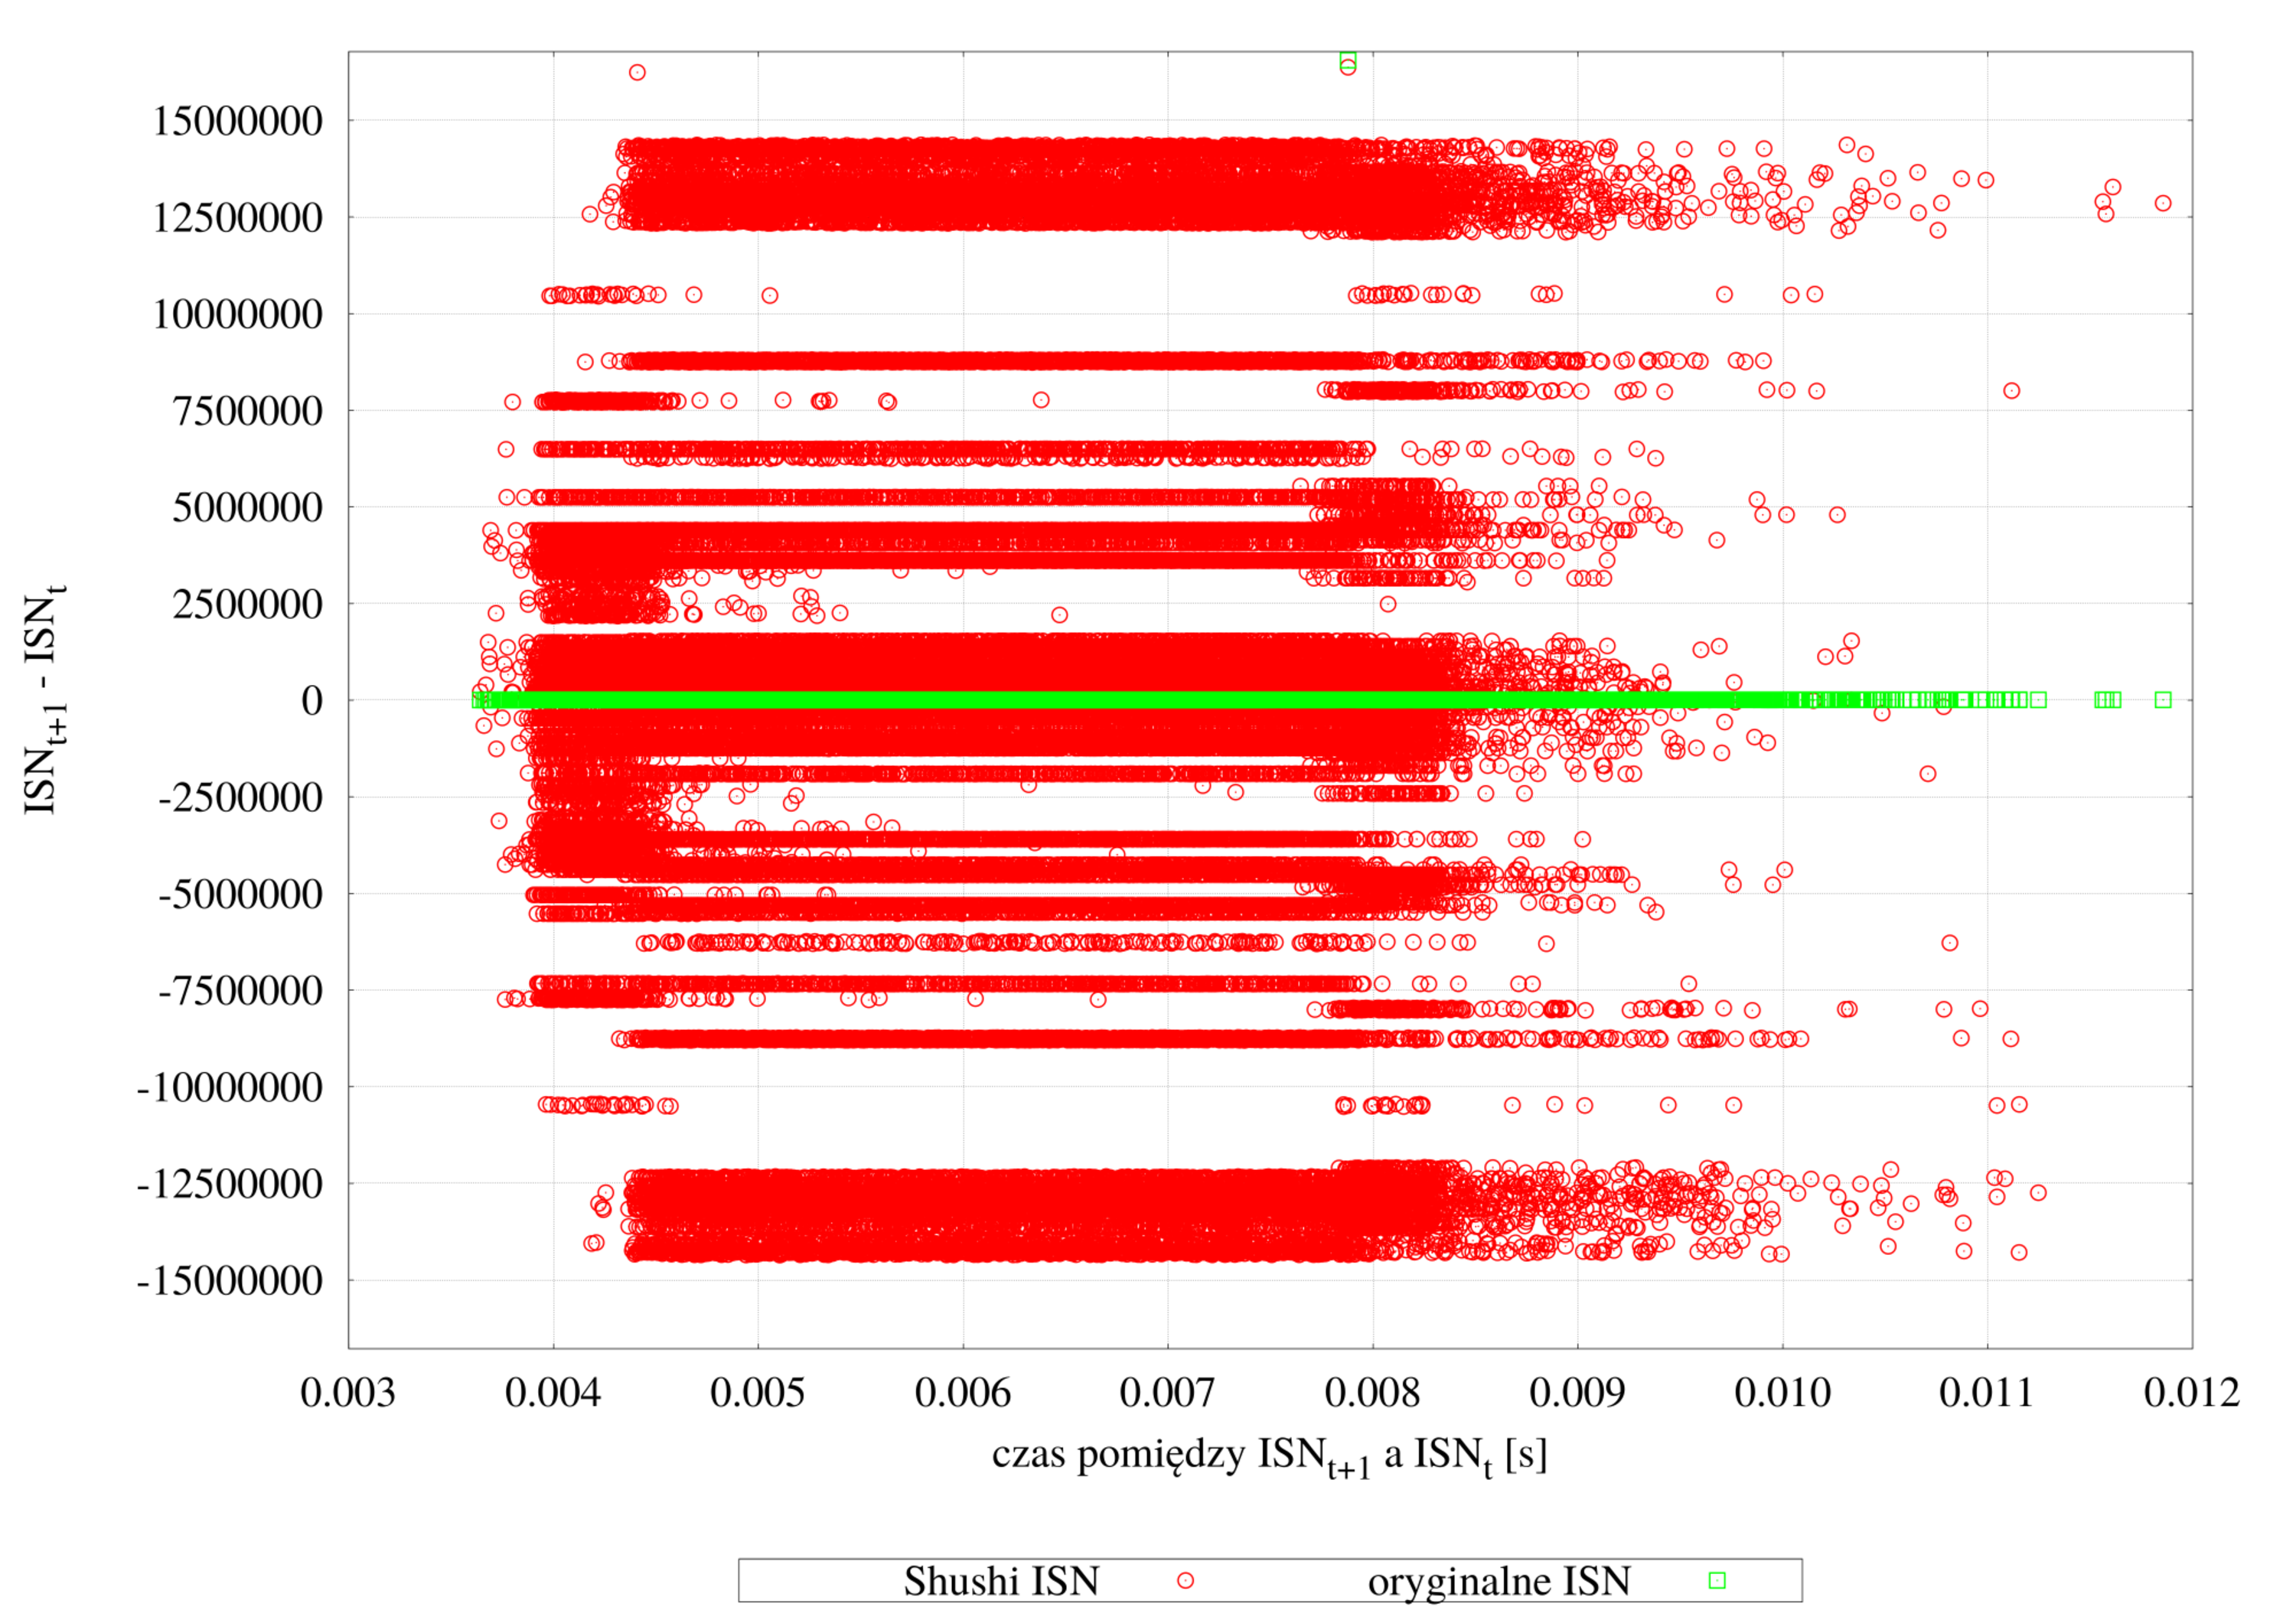
\includegraphics[scale=0.21]{\ImgPath/rys/IPPortConstDataDiff.pdf}
\end{center}
	\caption{Różnice pomiędzy kolejnymi numerami ISN wygenerowanymi przez 
jądro oraz \tech{Shushi}, stałe numery IP oraz porty TCP, stałe dane dla 
\tech{Shushi}, serie po około 60000 próbek.}
	\label{IPPortConstDataDiff}
\end{figure}


\begin{thebibliography}{99}
\addcontentsline{toc}{chapter}{Bibliografia}

\bibitem{KC}{Kodeks Cywilny,  Część Ogólna- Mienie  Art. 46.§ 1. https://isap.sejm.gov.pl/isap.nsf/download.xsp/WDU19640160093/U/D19640093Lj.pdf dost 27.09.2022}
\bibitem{RMRPiTegb}{ROZPORZĄDZENIE
MINISTRA ROZWOJU, PRACY I TECHNOLOGII1) z dnia 27 lipca 2021 r. w sprawie ewidencji gruntów i budynków, Złącznik 1}
\bibitem{Uopizp} {Dz. U. 2003 Nr 80 poz. 717, Ustawa z dnia 27 marca 2003 r. o planowaniu i zagospodarowaniu przestrzennym, Art. 2 pkt 12  https://isap.sejm.gov.pl/isap.nsf/download.xsp/WDU20030800717/U/D20030717Lj.pdf dost 27.09.2022}
\bibitem {Uogn}{ Dz.U. 1997 nr 115 poz. 741, Art. 4 pkt 3a,  Ustawa z dnia 21 sierpnia 1997 r. o gospodarce nieruchomościami, https://isap.sejm.gov.pl/isap.nsf/download.xsp/WDU19971150741/U/D19970741Lj.pdf, dost 27.09.2022}
\bibitem{RMI}{Dz.U. 2002 nr 75 poz. 690, Rozdz. 5, § 26. 1.Rozporządzenie Ministra Infrastruktury z dnia 12 kwietnia 2002 r. w sprawie warunków technicznych, jakim powinny odpowiadać budynki i ich usytuowanie, https://isap.sejm.gov.pl/isap.nsf/download.xsp/WDU20020750690/O/D20020690.pdf, dost 27.09.2022 }
\bibitem{Operat}{Obwieszczenie Marszałka Sejmu Rzeczypospolitej Polskiej z dnia 17 września 2021 r. w sprawie ogłoszenia jednolitego tekstu ustawy o gospodarce nieruchomościami ,Art. 156. 1, https://isap.sejm.gov.pl/isap.nsf/download.xsp/WDU20210001899/T/D20211899L.pdf dost 12.10.2022}
\bibitem{Operat2}{tamże, Art. 174 }

\bibitem{plfed}{Polska Federacji Stowarzyszeń Rzeczoznawców Majątkowych, Nowy Europejski Standard dot. Automatycznych Modeli Wyceny, https://pfsrm.pl/aktualnosci/item/480-nowy-europejski-standard-dot-automatycznych-modeli-wyceny, dost 17.10.2022}
\bibitem{AVMFigurska}{Marta Figurska, Automatyczne modele wyceny nieruchomości - ujęcie teoretyczne, Uniwersytet Warmińsko-Mazurski w Olsztynie,
https://www.researchgate.net/profile/Marta-Figurska-2/publication/325976006\_Automatyczne\_modele\_wyceny\_nieruchomosci\_-\_ujecie\_teoretyczne\_Automated\_valuation\_models\_on\_the\_real\_estate\_market\_-\_theoretical\_depiction/links/5b3218b74585150d23d4a616/Automatyczne-modele-wyceny-nieruchomosci-ujecie-teoretyczne-Automated-valuation-models-on-the-real-estate-market-theoretical-depiction.pdf dosy 17.10.2022
}
\bibitem{pricer}{https://pricer.pl/, dost 17.10.2022}
\bibitem{otodom}{https://pomoc.otodom.pl/hc/pl/articles/4403782095762-Mapa-cen-transakcji dost. 17.10.2022}
\bibitem{szybko}{https://ceny.szybko.pl/, dost 15.10.2022}
\bibitem{skup}{https://skup.io/darmowa-wycena-nieruchomosci/ dost 17.10.2022}
\bibitem{ceyszybko}{https://ceny.szybko.pl/wycena-nieruchomosci/sprzedaż/działka dost. 17.10.2022}
\bibitem{AVM} {European Valuation Standards , 9th Edition 2020, The European Group of Valuer's Associations, str 289, https://tegova.org/static/72fa037473e198cbd428e465158bcfdb/a6048c931cdc93\_TEGOVA\_EVS\_2020\_digital.pdf dost 14.10.2022}
\bibitem{AMVbilozor}{dr Małgorzata Renigier-Biłozor, prof Sabina Źróbek,  Marek Walacik,nAneta Chmielewska, Stosowanie AVM - aktualny temat dyskusji
praktyków i teoretyków związanych z gospodarką nieruchomościami}

\bibitem{OPRM}{Dz.U. 2021 poz. 555, Obwieszczenie Prezesa Rady Ministrów z dnia 3 marca 2021 r. w sprawie ogłoszenia jednolitego tekstu rozporządzenia Rady Ministrów w sprawie wyceny nieruchomości i sporządzania operatu szacunkowego, Rozdz.2 § 3.1, https://isap.sejm.gov.pl/isap.nsf/download.xsp/WDU20210000555/O/D20210555.pdf dost 27.09.2022}

\bibitem{UoGN}{Ustawa z dnia 21sierpnia 1997r.o gospodarce nieruchomościami; http://isap.sejm.gov.pl/isap.nsf/download.xsp/WDU20200001990/U/D20201990Lj.pdf}
\bibitem{UoP}{U S T A W Az dnia 27marca 2003r.o planowaniu izagospodarowaniu przestrzennym; http://isap.sejm.gov.pl/isap.nsf/download.xsp/WDU20210000741/U/D20210741Lj.pdf}

\bibitem{otodom_o_nas}{https://www.otodom.pl/pl/cennik/posrednicy-nieruchomosci dost 30.09.2022}




\end{thebibliography}

\zakonczenie  % wklejenie recenzji i opinii

\end{document}
%+++ END +++
